\section{Decision Algorithm}
\label{sec:algorithm}
 
The following subsections provide a detailed workflow of the solution discussed in [\textcolor{blue}{[CITE]}], along with an in-depth explanation of the components involved in this decision-making process.

\subsection{Decision Making Entity}

The Decision Making Entity, the cornerstone of our Energy Saving Solution, serves two primary functions: determining whether a cell should be considered for shutdown or bringup, and assessing the consequences of energy-saving decisions prior to modifying the network configuration. 
The decision-making process leverages real-time data and incorporates historical predictions from both the Traffic Predictor and Coverage Predictor.
The entity utilizes short-term throughput forecasts from the Traffic Predictor to determine whether a cell should be considered for shutdown based on the network's predicted throughput values.
The entity considers shutting down a cell if the throughput exceeds a certain threshold, and conversely, contemplates activating a cell if the throughput falls below this threshold.

After finalizing the decision to either activate or shut down a cell, the Coverage Predictor aids the entity in identifying the network sectors that can be deactivated with minimal service disruption. 
Once the control decision and its target cell are both confirmed, the entity uses the Digital Twin's simulations to assess the potential impact of the energy-saving policy before configuring the network via the SMO.
The overall functioning of this entity is defined in the procedure detailed in [\textcolor{blue}{[CITE]}]\\

\begin{algorithm} [t!]
    \caption{
        \texttt{Energy Saving Entity Algorithm},
    }
    \begin{algorithmic} [1]
        \Procedure{EnergySavingEntity}{\textsf{$\tau$, curr\_tpt, cqi\_curr, $\alpha_{th}$}}
            \State $\textsf{tpt\_pred} \gets \textsf{TrafficPredictor(curr\_tpt)}$
            \If{$\textsf{tpt\_pred} > \tau$}
                \State \# Cell shutdown procedure
                \State $\textsf{c\_map} \gets \textsf{CoveragePredictor()}$
                \State $\textsf{node} \gets \max(\textsf{c\_map})$ \Comment{Node with maximum $E_{ij}$ for given sector}
                \State Create \textsf{policy} for shutdown.
                \State $\textsf{policy} \gets \textsf{node}$
                \State $\textsf{cqi\_future} \gets \textsf{DigitalTwin(policy)}$
                \State $\alpha \gets \textsf{KL-Divergence}(\textsf{cqi\_future}, \textsf{cqi\_curr})$
                \If{$\alpha < \alpha_{th}$}
                    \State Transmit \textsf{policy}.
                \Else
                    \State Reinvoke \textsf{EnergySavingEntity($\tau$, curr\_tpt, cqi\_curr, $\alpha_{th}$)}.
                \EndIf
            \Else
                \State \# Cell bring-up procedure
                \ForAll{\textsf{nodes} switched off in the system}
                    \State Create \textsf{policy} to switch on node $n$.
                    \State $\textsf{cqi\_n} \gets \textsf{DigitalTwin(policy)}$
                    \State $\alpha_{n} \gets \textsf{KL-Divergence}(\textsf{cqi\_n}, \textsf{cqi\_curr})$
                \EndFor
                \State Select \textsf{finalPolicy} with $\min \left(\textsf{mod}(\alpha_{n} - \alpha_{th})\right)$.
                \State Transmit \textsf{finalPolicy}.
            \EndIf
        \EndProcedure
    \end{algorithmic}
    \label{alg:energy_saving_algo}
\end{algorithm}

\subsection{Traffic Prediction}
The Traffic Predictor estimates the net traffic volume for each sector as a function of time. 
This prediction is based on historical data and previous measurements. The Traffic Predictor uses pre-trained LSTM to forecast these values for the near-future. 
The model is itself trained on initial system data (initial 300 entries from NS3 simulator)
The inputs to the LSTM model are throughput, cell to which throughput belongs and the timestamp of the reading.
Every 1 hr, the model makes four fresh predictions (+15, +30, +45, +60)

There is no existing technology that can model the traffic in a network with 100\% accuracy. This is a known fact, which we can attribute to the stochastic nature of the traffic in the network.
Our approach emphasizes the use of a predictive model to accurately anticipate network traffic \textit{fluctuations}.
We establish a throughput threshold, beyond which network configurations require modification. 
The model is trained with the anticipation that it can guide us towards the appropriate direction of change, accounting for a certain degree of expected error.
To prevent altering our system's configarition based on an erroneous prediction, we use the Digital Twin to simulate the effects of the change before implementing it in the real network.  

We use an offline model for learning because using a pre-trained model with sufficient data does seem to suffice to predict traffic directions in our given setup.
Another reason, we do not use an online model is because traffic data varies irratically and not all the data we recieve is a scenario we want to model for.
\textcolor{blue}{In further versions of the solution, we plan to use an online learning model to update the model with real-time data.}
Keeping in that in mind, we performed a few experiments with different regression models and found that the LSTM model was the best fit for our requirements.
Our experiments and subsequents observations are detailed in [\textcolor{blue}{CITE}].

\subsection{Digital Twin}

The Digital Twin is a powerful tool for network management and optimization, as it allows operators to test and predict the effects of changes of a policy in a risk-free virtual environment before implementing it in a real network.
In the context of our solution, the Digital Twin is used to simulate a cellular network and is used to understand how the cell shutdown/bringup will affect the system overall. 
CloudRF [\textcolor{blue}{CITE}] is used to map out the area of service and simulate the power readings across it. 
The coverage area is represented as a 30 x 30 pixel grid, with power readings simulated for each individual pixel.
CloudRF generates predictions of the expected CQI distribution of the system using a Radio Link budget simulator.
This system is initialized with network inventory and predicted RF power (downlink) for each pixel from sectors which exceed the predefined threshold ($P_th$).

\subsection{Coverage Prediction}

\begin{algorithm} [t!]
    \caption{
        \texttt{\sysname pipeline flow}, 
        % \textit{Input:} 
        %     packet \textsf{pkt},
        %     current state \textsf{curr\_state},
        %     current round number \textsf{curr\_rd},
        %     operation mode \textsf{op\_mode},
        % \textit{Output:} 
        %     enncrypted/decrypted pkt \textsf{pkt'} 
    }
        \begin{algorithmic} [1]
            \Procedure{p4ead\_pipeline}{\textsf{pkt}, \textsf{curr\_state}, \textsf{curr\_rd}, \textsf{op\_mode}}
                \State prnd\_count $\gets$ 0
                \While{\textsf{prnd\_count} $<$ \textsf{RPP}} \label{algline:rpp}
                    \If{curr\_state == START}
                        \State curr\_state $\gets$ INIT
                        \State \textsf{pkt} $\gets$ \Call{INIT}{\textsf{pkt}}
                    \ElsIf{curr\_state == INIT}
                        \If{curr\_rd == 12}
                            \State curr\_state $\gets$ ABS\_AD
                            \State \textsf{pkt} $\gets$ \Call{AD\_ABS}{\textsf{pkt}}
                            \State curr\_rd $\gets$ 0
                        \EndIf
                    \ElsIf{curr\_state == ABS\_AD}
                        \If{curr\_rd == 6}
                            \State curr\_state $\gets$ ABS\_IP
                            \State \textsf{pkt} $\gets$ \Call{IP\_ABS}{\textsf{pkt}}
                            \State curr\_rd $\gets$ 0
                        \EndIf
                    \ElsIf{curr\_state == ABS\_IP}
                        \If{curr\_rd == 6}
                            \State curr\_state $\gets$ FINAL
                            \State curr\_rd $\gets$ 0
                        \EndIf
                    \ElsIf{curr\_state == FINAL}
                        \If{curr\_rd == 12}
                            \State curr\_state $\gets$ END
                            \State \textsf{pkt} $\gets$ \Call{TAG}{\textsf{pkt}}
                            \State \Call{break}{}   
                        \EndIf
                    \EndIf
                    \State \textsf{pkt} $\gets$ \Call{p\_rnd}{\textsf{pkt}}  \Comment{do one P-RND}
                    \State prnd\_count $\gets$ prnd\_count $+ 1$
                    \State curr\_rd $\gets$ curr\_rd $+ 1$
                \EndWhile
                \If{curr\_state == END}
                    \If{op\_mode == DECRYPT}
                        \State valid\_tag $\gets$ \Call{verify\_tag}{\textsf{pkt}}
                        \If{$\neg$valid\_tag}
                            \State \Call{drop}{\textsf{pkt}}
                        \EndIf
                    \EndIf
                    \State \textsf{pkt'} $\gets$ \textsf{pkt}
                    \State \Call{forward}{\textsf{pkt'}}
                \Else
                    \State \Call{recirculate}{\textsf{pkt}} 
                \EndIf
            \EndProcedure
        \end{algorithmic}
        \label{alg:pipeline}
    \end{algorithm}
    
     % \If {(cCount - \textsf{cms}.get\_count(flowId)) > $\sigma$} \label{algorithm_access_check_count_start}
     %                \State \textsf{pkt}.ctrl $\gets 0$ \COMMENT{prepare alert}
     %                \State \textsf{pkt}.dst\_ip $\gets$ \Call {Get\_Border\_IP}{\textsf{pkt}.ctrl.borderId}\label{algorithm_access_check_count_end}

     

The Coverage Predictor estimates the \textit{coverage overlap}, the areas where signals from neighboring sectors intersect. 
It identifies sectors that, if shut down, would not impact the overall network coverage. 
Sectors exhibiting the highest degree of overlap are prioritized for shutdown, given that their discontinuation is less likely to impact coverage due to the compensatory capabilities of the remaining interconnected sectors.

%It also updates the link level prediction model based on actual measured values to enhance accuracy. 
The system takes as input the simulated received power level (sourced from CloudRF) for each pixel from all sectors contributing more than $P_th$. 
The system outputs a matrix, known as a Coverage Map, which represents the degree of overlap between these sectors.$P_th$ of the system is a variable set depending on the environemnt in which the system is running. 
It depends on the sensitivity desired by the user and is set by the user.
The algorithm for the Coverage Predictor is detailed in Algorithm \textcolor{blue}{CITE} %\ref{alg:coverage_algo}.
$E_{ij}$ is the number of sectors which have overlaps with other sectors.

\textcolor{red}{[PRAMIT] - Could we represent this using a diagram of some sorts? Would be helpful.\\}

\subsection{Measuring  QoS Gurantees}


In the context of networking, Quality of Service (QoS) mainly involves guaranteeing a certain level of performance to a data flow. \textcolor{blue}{[https://dl.acm.org/doi/epdf/10.1145/173942.173943]} \\
In order to uphold QoS commitments in our system, it is essential to ensure that the implementation of energy-saving policies does not lead to a substantial decline in network performance.
This can be achieved by ensuring the system operates optimally at the outset and maintaining its initial state throughout. This principle guides our approach to monitoring system functioning.
Among these variables, the \textit{Channel Quality Indicator (CQI)} values of the active cells and the system's \texttt{total throughput} are of paramount importance.

Why don't we consider the throughput of each individual UE? Firstly, it's logistically impractical. 
UEs connect and disconnect from the network at a rapid pace, making it difficult and computationally intensive to track individual allotments.
Secondly, as long as the total system performance remains consistent with its state prior to control application, our initial Quality of Service (QoS) is assured.
\textcolor{blue}{While it's crucial to maintain a constant overall throughput, it's challenging to do so consistently, especially as network throughput tends to decrease when the network load is excessively high.}
Rather than focusing on individual metrics, we concentrate on measuring the system's Channel Quality Indicator (CQI) distribution. 
A low CQI value signifies poor channel quality, while a high CQI value signifies excellent channel quality. 
Our goal is to utilize high-quality channels. By consistently maintaining the use of such channels, we can ensure the preservation of the QoS to the users.

\begin{figure}[ht]
    \centering
    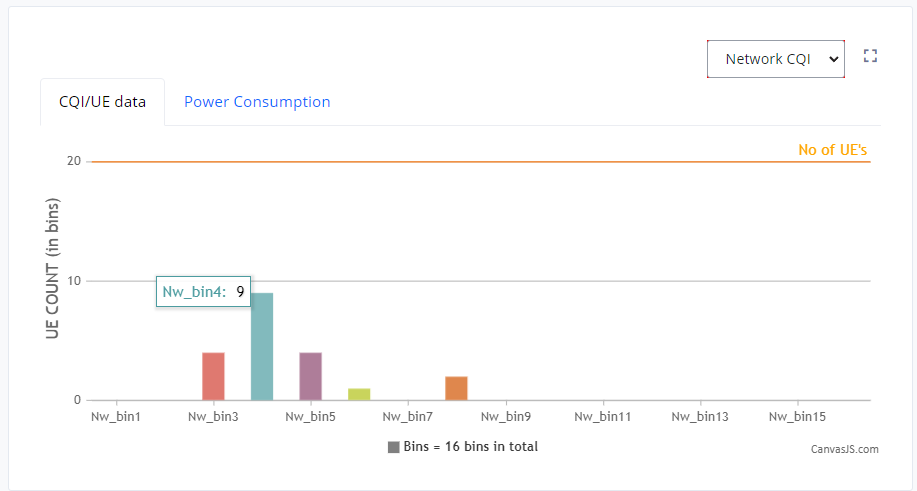
\includegraphics[width=0.4\textwidth]{/Users/pulakmehrotra/Desktop/SaankhyaLabs/es_oran_paper/acm_version_final/images/cqi_disrt.png}
    \caption{CQI Distribution}
    \label{fig:cqi_distr}
    \end{figure}

The overall system's CQI is measured by assigning each UE to a CQI-value 'bin', which is determined based on the channel quality measured by the core network.
\textcolor{blue}{The distribution of UEs across CQI bins closely mirrors a discrete probability distribution of CQI values across the network.}
We employ the Kullback-Leibler (KL) divergence, a statistical measure from information theory, to ensure that the input or output distributions do not deviate significantly from a baseline distribution \textcolor{blue}{[CITE]}.
The KL divergence of two probability distributions $P$ and $Q$ is defined as \textcolor{blue}{[CITE]}:

\begin{equation}
D_{KL}(P || Q) = \sum_{i} P(i) \log \frac{P(i)}{Q(i)}
\end{equation}

In this context, $P(i)$ and $Q(i)$ represent the probabilities of the $i$th CQI bin in the respective distributions $P$ and $Q$.

We derive the initial CQI distribution from the NS-3 simulator. 
Subsequently, the rApp policy is applied to generate a new network configuration, which is simulated in the Digital Twin to obtain a subsequent CQI distribution. 
The KL Divergence Function \textcolor{blue}{cite} is employed to compare these distributions. 
If the control policy does not induce a significant deviation from the baseline in the simulation, it is then relayed to the Near-RT RIC. 
The user sets the difference threshold, $\alpha_{th}$, which varies based on the specific situation.

